% Options for packages loaded elsewhere
\PassOptionsToPackage{unicode}{hyperref}
\PassOptionsToPackage{hyphens}{url}
%
\documentclass[
]{article}
\usepackage{amsmath,amssymb}
\usepackage{iftex}
\ifPDFTeX
  \usepackage[T1]{fontenc}
  \usepackage[utf8]{inputenc}
  \usepackage{textcomp} % provide euro and other symbols
\else % if luatex or xetex
  \usepackage{unicode-math} % this also loads fontspec
  \defaultfontfeatures{Scale=MatchLowercase}
  \defaultfontfeatures[\rmfamily]{Ligatures=TeX,Scale=1}
\fi
\usepackage{lmodern}
\ifPDFTeX\else
  % xetex/luatex font selection
\fi
% Use upquote if available, for straight quotes in verbatim environments
\IfFileExists{upquote.sty}{\usepackage{upquote}}{}
\IfFileExists{microtype.sty}{% use microtype if available
  \usepackage[]{microtype}
  \UseMicrotypeSet[protrusion]{basicmath} % disable protrusion for tt fonts
}{}
\makeatletter
\@ifundefined{KOMAClassName}{% if non-KOMA class
  \IfFileExists{parskip.sty}{%
    \usepackage{parskip}
  }{% else
    \setlength{\parindent}{0pt}
    \setlength{\parskip}{6pt plus 2pt minus 1pt}}
}{% if KOMA class
  \KOMAoptions{parskip=half}}
\makeatother
\usepackage{xcolor}
\usepackage[margin=1in]{geometry}
\usepackage{color}
\usepackage{fancyvrb}
\newcommand{\VerbBar}{|}
\newcommand{\VERB}{\Verb[commandchars=\\\{\}]}
\DefineVerbatimEnvironment{Highlighting}{Verbatim}{commandchars=\\\{\}}
% Add ',fontsize=\small' for more characters per line
\usepackage{framed}
\definecolor{shadecolor}{RGB}{248,248,248}
\newenvironment{Shaded}{\begin{snugshade}}{\end{snugshade}}
\newcommand{\AlertTok}[1]{\textcolor[rgb]{0.94,0.16,0.16}{#1}}
\newcommand{\AnnotationTok}[1]{\textcolor[rgb]{0.56,0.35,0.01}{\textbf{\textit{#1}}}}
\newcommand{\AttributeTok}[1]{\textcolor[rgb]{0.13,0.29,0.53}{#1}}
\newcommand{\BaseNTok}[1]{\textcolor[rgb]{0.00,0.00,0.81}{#1}}
\newcommand{\BuiltInTok}[1]{#1}
\newcommand{\CharTok}[1]{\textcolor[rgb]{0.31,0.60,0.02}{#1}}
\newcommand{\CommentTok}[1]{\textcolor[rgb]{0.56,0.35,0.01}{\textit{#1}}}
\newcommand{\CommentVarTok}[1]{\textcolor[rgb]{0.56,0.35,0.01}{\textbf{\textit{#1}}}}
\newcommand{\ConstantTok}[1]{\textcolor[rgb]{0.56,0.35,0.01}{#1}}
\newcommand{\ControlFlowTok}[1]{\textcolor[rgb]{0.13,0.29,0.53}{\textbf{#1}}}
\newcommand{\DataTypeTok}[1]{\textcolor[rgb]{0.13,0.29,0.53}{#1}}
\newcommand{\DecValTok}[1]{\textcolor[rgb]{0.00,0.00,0.81}{#1}}
\newcommand{\DocumentationTok}[1]{\textcolor[rgb]{0.56,0.35,0.01}{\textbf{\textit{#1}}}}
\newcommand{\ErrorTok}[1]{\textcolor[rgb]{0.64,0.00,0.00}{\textbf{#1}}}
\newcommand{\ExtensionTok}[1]{#1}
\newcommand{\FloatTok}[1]{\textcolor[rgb]{0.00,0.00,0.81}{#1}}
\newcommand{\FunctionTok}[1]{\textcolor[rgb]{0.13,0.29,0.53}{\textbf{#1}}}
\newcommand{\ImportTok}[1]{#1}
\newcommand{\InformationTok}[1]{\textcolor[rgb]{0.56,0.35,0.01}{\textbf{\textit{#1}}}}
\newcommand{\KeywordTok}[1]{\textcolor[rgb]{0.13,0.29,0.53}{\textbf{#1}}}
\newcommand{\NormalTok}[1]{#1}
\newcommand{\OperatorTok}[1]{\textcolor[rgb]{0.81,0.36,0.00}{\textbf{#1}}}
\newcommand{\OtherTok}[1]{\textcolor[rgb]{0.56,0.35,0.01}{#1}}
\newcommand{\PreprocessorTok}[1]{\textcolor[rgb]{0.56,0.35,0.01}{\textit{#1}}}
\newcommand{\RegionMarkerTok}[1]{#1}
\newcommand{\SpecialCharTok}[1]{\textcolor[rgb]{0.81,0.36,0.00}{\textbf{#1}}}
\newcommand{\SpecialStringTok}[1]{\textcolor[rgb]{0.31,0.60,0.02}{#1}}
\newcommand{\StringTok}[1]{\textcolor[rgb]{0.31,0.60,0.02}{#1}}
\newcommand{\VariableTok}[1]{\textcolor[rgb]{0.00,0.00,0.00}{#1}}
\newcommand{\VerbatimStringTok}[1]{\textcolor[rgb]{0.31,0.60,0.02}{#1}}
\newcommand{\WarningTok}[1]{\textcolor[rgb]{0.56,0.35,0.01}{\textbf{\textit{#1}}}}
\usepackage{graphicx}
\makeatletter
\def\maxwidth{\ifdim\Gin@nat@width>\linewidth\linewidth\else\Gin@nat@width\fi}
\def\maxheight{\ifdim\Gin@nat@height>\textheight\textheight\else\Gin@nat@height\fi}
\makeatother
% Scale images if necessary, so that they will not overflow the page
% margins by default, and it is still possible to overwrite the defaults
% using explicit options in \includegraphics[width, height, ...]{}
\setkeys{Gin}{width=\maxwidth,height=\maxheight,keepaspectratio}
% Set default figure placement to htbp
\makeatletter
\def\fps@figure{htbp}
\makeatother
\setlength{\emergencystretch}{3em} % prevent overfull lines
\providecommand{\tightlist}{%
  \setlength{\itemsep}{0pt}\setlength{\parskip}{0pt}}
\setcounter{secnumdepth}{-\maxdimen} % remove section numbering
\usepackage{fontspec}
\setmainfont{Times New Roman}
\usepackage{ctex}
\ifLuaTeX
  \usepackage{selnolig}  % disable illegal ligatures
\fi
\usepackage{bookmark}
\IfFileExists{xurl.sty}{\usepackage{xurl}}{} % add URL line breaks if available
\urlstyle{same}
\hypersetup{
  pdftitle={homework4},
  pdfauthor={黄舟翔 3220103606},
  hidelinks,
  pdfcreator={LaTeX via pandoc}}

\title{homework4}
\author{黄舟翔 3220103606}
\date{2025-06-29}

\begin{document}
\maketitle

We continue examining the diffusion of tetracycline among doctors in
Illinois in the early 1950s, building on our work in lab 6. You will
need the data sets \texttt{ckm\_nodes.csv} and \texttt{ckm\_network.dat}
from the labs.

\subsubsection{1.}\label{section}

Clean the data to eliminate doctors for whom we have no adoption-date
information, as in the labs. Only use this cleaned data in the rest of
the assignment.

用以下代码完成:

\begin{Shaded}
\begin{Highlighting}[]
\NormalTok{ckm\_nodes }\OtherTok{\textless{}{-}} \FunctionTok{read\_csv}\NormalTok{(}\StringTok{\textquotesingle{}data/ckm\_nodes.csv\textquotesingle{}}\NormalTok{)}
\NormalTok{noinfor }\OtherTok{\textless{}{-}} \FunctionTok{which}\NormalTok{(}\FunctionTok{is.na}\NormalTok{(ckm\_nodes}\SpecialCharTok{$}\NormalTok{adoption\_date))}
\NormalTok{ckm\_nodes }\OtherTok{\textless{}{-}}\NormalTok{ ckm\_nodes[}\SpecialCharTok{{-}}\NormalTok{noinfor, ]}
\NormalTok{ckm\_network }\OtherTok{\textless{}{-}} \FunctionTok{read.table}\NormalTok{(}\StringTok{\textquotesingle{}data/ckm\_network.dat\textquotesingle{}}\NormalTok{)}
\NormalTok{ckm\_network }\OtherTok{\textless{}{-}}\NormalTok{ ckm\_network[}\SpecialCharTok{{-}}\NormalTok{noinfor, }\SpecialCharTok{{-}}\NormalTok{noinfor]}
\end{Highlighting}
\end{Shaded}

\subsubsection{2.}\label{section-1}

Create a new data frame which records, for every doctor, for every
month, whether that doctor began prescribing tetracycline that month,
whether they had adopted tetracycline before that month, the number of
their contacts who began prescribing strictly \emph{before} that month,
and the number of their contacts who began prescribing in that month or
earlier. Explain why the dataframe should have 6 columns, and 2125 rows.

用以下代码完成:

\begin{Shaded}
\begin{Highlighting}[]
\NormalTok{ckm\_nodes }\OtherTok{\textless{}{-}}\NormalTok{ ckm\_nodes }\SpecialCharTok{\%\textgreater{}\%} 
  \FunctionTok{mutate}\NormalTok{(}\AttributeTok{id =} \FunctionTok{row\_number}\NormalTok{())}

\CommentTok{\# 2. 创建新数据框}
\NormalTok{doctors }\OtherTok{\textless{}{-}}\NormalTok{ ckm\_nodes}\SpecialCharTok{$}\NormalTok{id}
\NormalTok{months }\OtherTok{\textless{}{-}} \DecValTok{1}\SpecialCharTok{:}\DecValTok{17}

\CommentTok{\# 创建医生与月份的所有组合}
\NormalTok{df }\OtherTok{\textless{}{-}} \FunctionTok{expand\_grid}\NormalTok{(}\AttributeTok{doctor =}\NormalTok{ doctors, }\AttributeTok{month =}\NormalTok{ months)}

\CommentTok{\# 添加医生的采用日期}
\NormalTok{df }\OtherTok{\textless{}{-}}\NormalTok{ df }\SpecialCharTok{\%\textgreater{}\%} 
  \FunctionTok{left\_join}\NormalTok{(}\FunctionTok{select}\NormalTok{(ckm\_nodes, id, adoption\_date), }\AttributeTok{by =} \FunctionTok{c}\NormalTok{(}\StringTok{"doctor"} \OtherTok{=} \StringTok{"id"}\NormalTok{))}

\CommentTok{\# 创建采用指标列}
\NormalTok{df }\OtherTok{\textless{}{-}}\NormalTok{ df }\SpecialCharTok{\%\textgreater{}\%}
  \FunctionTok{mutate}\NormalTok{(}
    \AttributeTok{adopted =} \FunctionTok{as.integer}\NormalTok{(adoption\_date }\SpecialCharTok{==}\NormalTok{ month),}
    \AttributeTok{before\_adopted =} \FunctionTok{as.integer}\NormalTok{(adoption\_date }\SpecialCharTok{\textless{}}\NormalTok{ month)}
\NormalTok{  )}

\CommentTok{\# 预计算每位医生的联系人采用日期}
\NormalTok{contact\_adopters }\OtherTok{\textless{}{-}} \FunctionTok{apply}\NormalTok{(ckm\_network, }\DecValTok{1}\NormalTok{, }\ControlFlowTok{function}\NormalTok{(row) \{}
\NormalTok{  contacts }\OtherTok{\textless{}{-}} \FunctionTok{which}\NormalTok{(row }\SpecialCharTok{\textgreater{}} \DecValTok{0}\NormalTok{)}
\NormalTok{  ckm\_nodes}\SpecialCharTok{$}\NormalTok{adoption\_date[contacts]}
\NormalTok{\})}

\CommentTok{\# 计算联系人采用数量的函数}
\NormalTok{calculate\_contacts }\OtherTok{\textless{}{-}} \ControlFlowTok{function}\NormalTok{(doctor\_index, current\_month) \{}
\NormalTok{  contact\_dates }\OtherTok{\textless{}{-}}\NormalTok{ contact\_adopters[[doctor\_index]]}
\NormalTok{  contacts\_before }\OtherTok{\textless{}{-}} \FunctionTok{sum}\NormalTok{(contact\_dates }\SpecialCharTok{\textless{}}\NormalTok{ current\_month, }\AttributeTok{na.rm =} \ConstantTok{TRUE}\NormalTok{)}
\NormalTok{  contacts\_at\_or\_before }\OtherTok{\textless{}{-}} \FunctionTok{sum}\NormalTok{(contact\_dates }\SpecialCharTok{\textless{}=}\NormalTok{ current\_month, }\AttributeTok{na.rm =} \ConstantTok{TRUE}\NormalTok{)}
  \FunctionTok{data.frame}\NormalTok{(}
    \AttributeTok{count\_contacts\_before =}\NormalTok{ contacts\_before,}
    \AttributeTok{count\_contacts\_at\_or\_before =}\NormalTok{ contacts\_at\_or\_before}
\NormalTok{  )}
\NormalTok{\}}

\CommentTok{\# 为每行数据计算联系人指标}
\NormalTok{contact\_counts }\OtherTok{\textless{}{-}} \FunctionTok{map2\_dfr}\NormalTok{(}
  \AttributeTok{.x =} \FunctionTok{match}\NormalTok{(df}\SpecialCharTok{$}\NormalTok{doctor, doctors),}
  \AttributeTok{.y =}\NormalTok{ df}\SpecialCharTok{$}\NormalTok{month,}
  \AttributeTok{.f =} \SpecialCharTok{\textasciitilde{}} \FunctionTok{calculate\_contacts}\NormalTok{(.x, .y)}
\NormalTok{)}

\CommentTok{\# 合并到主数据框}
\NormalTok{df }\OtherTok{\textless{}{-}} \FunctionTok{bind\_cols}\NormalTok{(df, contact\_counts) }\SpecialCharTok{\%\textgreater{}\%}
  \FunctionTok{select}\NormalTok{(}\SpecialCharTok{{-}}\NormalTok{adoption\_date)}

\CommentTok{\# 验证数据框结构}
\FunctionTok{cat}\NormalTok{(}\StringTok{"行数:"}\NormalTok{, }\FunctionTok{nrow}\NormalTok{(df), }\StringTok{"(应为125医生×17月=2125)}\SpecialCharTok{\textbackslash{}n}\StringTok{"}\NormalTok{)}
\end{Highlighting}
\end{Shaded}

\begin{verbatim}
## 行数: 2125 (应为125医生×17月=2125)
\end{verbatim}

\begin{Shaded}
\begin{Highlighting}[]
\FunctionTok{cat}\NormalTok{(}\StringTok{"列数:"}\NormalTok{, }\FunctionTok{ncol}\NormalTok{(df), }\StringTok{"(应为6)}\SpecialCharTok{\textbackslash{}n}\StringTok{"}\NormalTok{)}
\end{Highlighting}
\end{Shaded}

\begin{verbatim}
## 列数: 6 (应为6)
\end{verbatim}

\begin{Shaded}
\begin{Highlighting}[]
\FunctionTok{cat}\NormalTok{(}\StringTok{"列名:"}\NormalTok{, }\FunctionTok{paste}\NormalTok{(}\FunctionTok{colnames}\NormalTok{(df), }\AttributeTok{collapse =} \StringTok{", "}\NormalTok{), }\StringTok{"}\SpecialCharTok{\textbackslash{}n}\StringTok{"}\NormalTok{)}
\end{Highlighting}
\end{Shaded}

\begin{verbatim}
## 列名: doctor, month, adopted, before_adopted, count_contacts_before, count_contacts_at_or_before
\end{verbatim}

\subsubsection{3.}\label{section-2}

Let

    \begin{equation}
    \begin{split}
    p_k & = \Pr(\text{A doctor starts prescribing tetracycline this month} \mid \\
     & \text{Number of doctor's contacts prescribing before this month}=k) 
     \end{split}
     \end{equation}

and

    \begin{equation}
    \begin{split}
     q_k & = \Pr(\text{A doctor starts prescribing tetracycline this month} \mid \\ 
     & \text{Number of doctor's contacts prescribing this month}=k)
     \end{split}
     \end{equation}

We suppose that \(p_k\) and \(q_k\) are the same for all months.

\paragraph{a.}\label{a.}

Explain why there should be no more than \(21\) values of \(k\) for
which we can estimate \(p_k\) and \(q_k\) directly from the data.

每个医生的联系人数量(度数)是有限的,一个医生最多有 20 个联系人。

k 的可能取值范围:k 表示已采用的联系人数量,其取值范围为 0 到最大度数

k = 0, 1, 2, \ldots, 20 → 共 21 个可能取值

对于 k \textgreater{} 20 的情况,数据集中不存在这样的医生

因此,我们最多只能直接估计 21 个 k 值对应的 \(p_k\) 和 \(q_k\) 概率

\paragraph{b.}\label{b.}

Create a vector of estimated \(p_k\) probabilities, using the data frame
from (2). Plot the probabilities against the number of prior-adoptee
contacts \(k\).

用以下代码解决

\begin{Shaded}
\begin{Highlighting}[]
\CommentTok{\# 计算 p\_k}
\NormalTok{p\_data }\OtherTok{\textless{}{-}}\NormalTok{ df }\SpecialCharTok{\%\textgreater{}\%}
  \FunctionTok{filter}\NormalTok{(before\_adopted }\SpecialCharTok{==} \DecValTok{0}\NormalTok{) }\SpecialCharTok{\%\textgreater{}\%}  \CommentTok{\# 只考虑本月前未采用的医生}
  \FunctionTok{group\_by}\NormalTok{(count\_contacts\_before) }\SpecialCharTok{\%\textgreater{}\%}  \CommentTok{\# 按 k 分组}
  \FunctionTok{summarise}\NormalTok{(}
    \AttributeTok{n =} \FunctionTok{n}\NormalTok{(),  }\CommentTok{\# 该 k 值的总医生数}
    \AttributeTok{adopted\_this\_month =} \FunctionTok{sum}\NormalTok{(adopted),  }\CommentTok{\# 本月采用的医生数}
    \AttributeTok{p\_k =}\NormalTok{ adopted\_this\_month }\SpecialCharTok{/}\NormalTok{ n  }\CommentTok{\# 概率估计}
\NormalTok{  ) }\SpecialCharTok{\%\textgreater{}\%}
  \FunctionTok{rename}\NormalTok{(}\AttributeTok{k =}\NormalTok{ count\_contacts\_before)  }\CommentTok{\# 重命名列}

\CommentTok{\# 绘制 p\_k}
\FunctionTok{ggplot}\NormalTok{(p\_data, }\FunctionTok{aes}\NormalTok{(}\AttributeTok{x =}\NormalTok{ k, }\AttributeTok{y =}\NormalTok{ p\_k)) }\SpecialCharTok{+}
  \FunctionTok{geom\_point}\NormalTok{(}\AttributeTok{size =} \DecValTok{3}\NormalTok{, }\AttributeTok{color =} \StringTok{"blue"}\NormalTok{) }\SpecialCharTok{+}
  \FunctionTok{geom\_smooth}\NormalTok{(}\AttributeTok{method =} \StringTok{"loess"}\NormalTok{, }\AttributeTok{se =} \ConstantTok{FALSE}\NormalTok{, }\AttributeTok{color =} \StringTok{"darkblue"}\NormalTok{, }\AttributeTok{linetype =} \StringTok{"dashed"}\NormalTok{) }\SpecialCharTok{+}
  \FunctionTok{labs}\NormalTok{(}
    \AttributeTok{title =} \StringTok{"The relationship between adoption probability and the number of previously adopted contacts before the current month"}\NormalTok{,}
    \AttributeTok{subtitle =} \FunctionTok{expression}\NormalTok{(}\FunctionTok{paste}\NormalTok{(}\StringTok{"estimated "}\NormalTok{, p[k], }\StringTok{" probability"}\NormalTok{)),}
    \AttributeTok{x =} \StringTok{"Number of contacts adopted prior to this month (k)"}\NormalTok{,}
    \AttributeTok{y =} \FunctionTok{expression}\NormalTok{(p[k])}
\NormalTok{  ) }\SpecialCharTok{+}
  \FunctionTok{theme\_minimal}\NormalTok{(}\AttributeTok{base\_size =} \DecValTok{12}\NormalTok{) }\SpecialCharTok{+}
  \FunctionTok{theme}\NormalTok{(}\AttributeTok{plot.title =} \FunctionTok{element\_text}\NormalTok{(}\AttributeTok{hjust =} \FloatTok{0.5}\NormalTok{)) }\SpecialCharTok{+}
  \FunctionTok{scale\_x\_continuous}\NormalTok{(}\AttributeTok{breaks =} \FunctionTok{seq}\NormalTok{(}\DecValTok{0}\NormalTok{, }\DecValTok{20}\NormalTok{, }\AttributeTok{by =} \DecValTok{2}\NormalTok{)) }\SpecialCharTok{+}
  \FunctionTok{ylim}\NormalTok{(}\DecValTok{0}\NormalTok{, }\FloatTok{0.5}\NormalTok{)  }\CommentTok{\# 根据实际数据范围调整}
\end{Highlighting}
\end{Shaded}

\begin{verbatim}
## `geom_smooth()` using formula = 'y ~ x'
\end{verbatim}

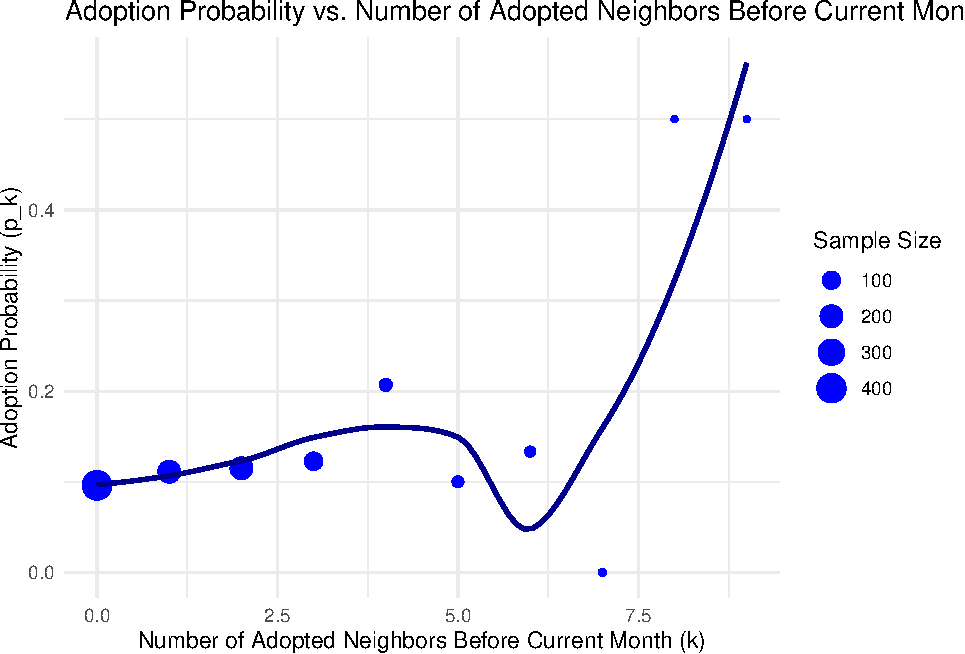
\includegraphics{Homework-04_files/figure-latex/unnamed-chunk-3-1.pdf}
\#\#\#\# c.~

Create a vector of estimated \(q_k\) probabilities, using the data frame
from (2). Plot the probabilities against the number of
prior-or-contemporary-adoptee contacts \(k\).

用以下代码解决

\begin{Shaded}
\begin{Highlighting}[]
\CommentTok{\# 计算 q\_k}
\NormalTok{q\_data }\OtherTok{\textless{}{-}}\NormalTok{ df }\SpecialCharTok{\%\textgreater{}\%}
  \FunctionTok{filter}\NormalTok{(before\_adopted }\SpecialCharTok{==} \DecValTok{0}\NormalTok{) }\SpecialCharTok{\%\textgreater{}\%}  \CommentTok{\# 只考虑本月前未采用的医生}
  \FunctionTok{group\_by}\NormalTok{(count\_contacts\_at\_or\_before) }\SpecialCharTok{\%\textgreater{}\%}  \CommentTok{\# 按 k 分组}
  \FunctionTok{summarise}\NormalTok{(}
    \AttributeTok{n =} \FunctionTok{n}\NormalTok{(),  }\CommentTok{\# 该 k 值的总医生数}
    \AttributeTok{adopted\_this\_month =} \FunctionTok{sum}\NormalTok{(adopted),  }\CommentTok{\# 本月采用的医生数}
    \AttributeTok{q\_k =}\NormalTok{ adopted\_this\_month }\SpecialCharTok{/}\NormalTok{ n  }\CommentTok{\# 概率估计}
\NormalTok{  ) }\SpecialCharTok{\%\textgreater{}\%}
  \FunctionTok{rename}\NormalTok{(}\AttributeTok{k =}\NormalTok{ count\_contacts\_at\_or\_before)  }\CommentTok{\# 重命名列}

\CommentTok{\# 绘制 q\_k}
\FunctionTok{ggplot}\NormalTok{(q\_data, }\FunctionTok{aes}\NormalTok{(}\AttributeTok{x =}\NormalTok{ k, }\AttributeTok{y =}\NormalTok{ q\_k)) }\SpecialCharTok{+}
  \FunctionTok{geom\_point}\NormalTok{(}\AttributeTok{size =} \DecValTok{3}\NormalTok{, }\AttributeTok{color =} \StringTok{"red"}\NormalTok{) }\SpecialCharTok{+}
  \FunctionTok{geom\_smooth}\NormalTok{(}\AttributeTok{method =} \StringTok{"loess"}\NormalTok{, }\AttributeTok{se =} \ConstantTok{FALSE}\NormalTok{, }\AttributeTok{color =} \StringTok{"darkred"}\NormalTok{, }\AttributeTok{linetype =} \StringTok{"dashed"}\NormalTok{) }\SpecialCharTok{+}
  \FunctionTok{labs}\NormalTok{(}
    \AttributeTok{title =} \StringTok{"The relationship between adoption probability and the number of contacts already adopted this month or previously"}\NormalTok{,}
    \AttributeTok{subtitle =} \FunctionTok{expression}\NormalTok{(}\FunctionTok{paste}\NormalTok{(}\StringTok{"estimated "}\NormalTok{, q[k], }\StringTok{" probability"}\NormalTok{)),}
    \AttributeTok{x =} \StringTok{"Number of contacts already adopted this month or earlier (k)"}\NormalTok{,}
    \AttributeTok{y =} \FunctionTok{expression}\NormalTok{(q[k])}
\NormalTok{  ) }\SpecialCharTok{+}
  \FunctionTok{theme\_minimal}\NormalTok{(}\AttributeTok{base\_size =} \DecValTok{12}\NormalTok{) }\SpecialCharTok{+}
  \FunctionTok{theme}\NormalTok{(}\AttributeTok{plot.title =} \FunctionTok{element\_text}\NormalTok{(}\AttributeTok{hjust =} \FloatTok{0.5}\NormalTok{)) }\SpecialCharTok{+}
  \FunctionTok{scale\_x\_continuous}\NormalTok{(}\AttributeTok{breaks =} \FunctionTok{seq}\NormalTok{(}\DecValTok{0}\NormalTok{, }\DecValTok{20}\NormalTok{, }\AttributeTok{by =} \DecValTok{2}\NormalTok{)) }\SpecialCharTok{+}
  \FunctionTok{ylim}\NormalTok{(}\DecValTok{0}\NormalTok{, }\FloatTok{0.5}\NormalTok{)  }\CommentTok{\# 根据实际数据范围调整}
\end{Highlighting}
\end{Shaded}

\begin{verbatim}
## `geom_smooth()` using formula = 'y ~ x'
\end{verbatim}

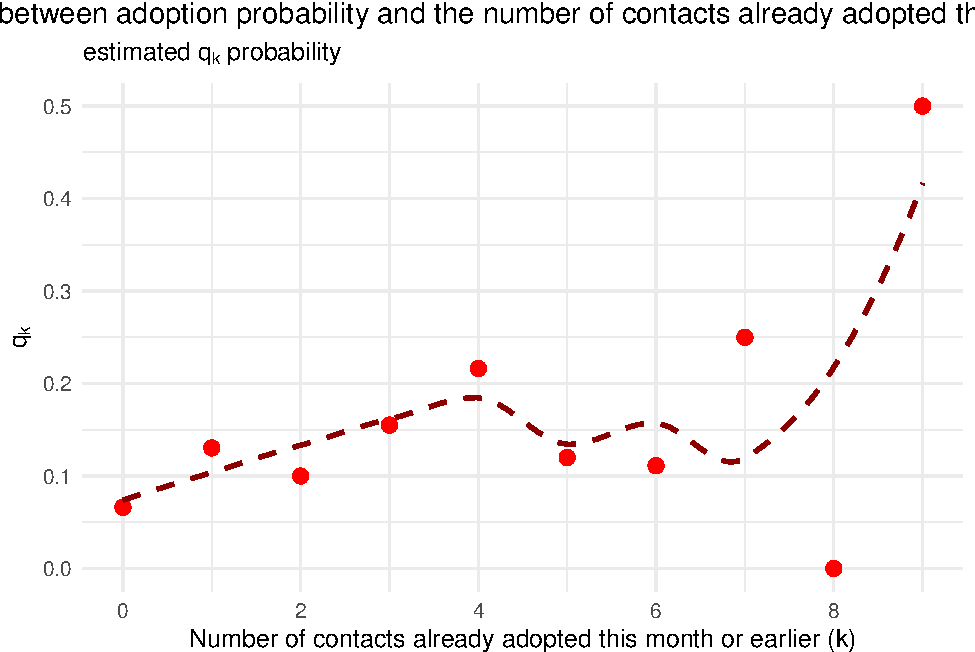
\includegraphics{Homework-04_files/figure-latex/unnamed-chunk-4-1.pdf}

\subsubsection{4.}\label{section-3}

Because it only conditions on information from the previous month,
\(p_k\) is a little easier to interpret than \(q_k\). It is the
probability per month that a doctor adopts tetracycline, if they have
exactly \(k\) contacts who had already adopted tetracycline.

\paragraph{a.}\label{a.-1}

Suppose \(p_k = a + bk\). This would mean that each friend who adopts
the new drug increases the probability of adoption by an equal amount.
Estimate this model by least squares, using the values you constructed
in (3b). Report the parameter estimates.

用以下代码解决:

\begin{Shaded}
\begin{Highlighting}[]
\CommentTok{\# 确保 p\_data 存在}
\ControlFlowTok{if}\NormalTok{ (}\SpecialCharTok{!}\FunctionTok{exists}\NormalTok{(}\StringTok{"p\_data"}\NormalTok{)) \{}
  \FunctionTok{stop}\NormalTok{(}\StringTok{"p\_data 未定义,请先执行问题3b的代码"}\NormalTok{)}
\NormalTok{\}}

\CommentTok{\# 拟合线性模型}
\NormalTok{linear\_model }\OtherTok{\textless{}{-}} \FunctionTok{lm}\NormalTok{(p\_k }\SpecialCharTok{\textasciitilde{}}\NormalTok{ k, }\AttributeTok{data =}\NormalTok{ p\_data)}

\CommentTok{\# 获取参数估计}
\NormalTok{a\_linear }\OtherTok{\textless{}{-}} \FunctionTok{coef}\NormalTok{(linear\_model)[}\DecValTok{1}\NormalTok{]}
\NormalTok{b\_linear }\OtherTok{\textless{}{-}} \FunctionTok{coef}\NormalTok{(linear\_model)[}\DecValTok{2}\NormalTok{]}

\CommentTok{\# 输出参数估计}
\FunctionTok{cat}\NormalTok{(}\StringTok{"Linear model parameter estimates:}\SpecialCharTok{\textbackslash{}n}\StringTok{"}\NormalTok{)}
\end{Highlighting}
\end{Shaded}

\begin{verbatim}
## Linear model parameter estimates:
\end{verbatim}

\begin{Shaded}
\begin{Highlighting}[]
\FunctionTok{cat}\NormalTok{(}\FunctionTok{sprintf}\NormalTok{(}\StringTok{"Intercept a = \%.4f}\SpecialCharTok{\textbackslash{}n}\StringTok{"}\NormalTok{, a\_linear))}
\end{Highlighting}
\end{Shaded}

\begin{verbatim}
## Intercept a = 0.0328
\end{verbatim}

\begin{Shaded}
\begin{Highlighting}[]
\FunctionTok{cat}\NormalTok{(}\FunctionTok{sprintf}\NormalTok{(}\StringTok{"Slope b = \%.4f}\SpecialCharTok{\textbackslash{}n}\StringTok{"}\NormalTok{, b\_linear))}
\end{Highlighting}
\end{Shaded}

\begin{verbatim}
## Slope b = 0.0346
\end{verbatim}

\begin{Shaded}
\begin{Highlighting}[]
\CommentTok{\# 创建可视化}
\FunctionTok{ggplot}\NormalTok{(p\_data, }\FunctionTok{aes}\NormalTok{(}\AttributeTok{x =}\NormalTok{ k, }\AttributeTok{y =}\NormalTok{ p\_k)) }\SpecialCharTok{+}
  \CommentTok{\# 原始数据点}
  \FunctionTok{geom\_point}\NormalTok{(}\AttributeTok{size =} \DecValTok{3}\NormalTok{, }\AttributeTok{color =} \StringTok{"steelblue"}\NormalTok{, }\AttributeTok{alpha =} \FloatTok{0.8}\NormalTok{) }\SpecialCharTok{+}
  \CommentTok{\# 线性拟合线}
  \FunctionTok{geom\_smooth}\NormalTok{(}
    \AttributeTok{method =} \StringTok{"lm"}\NormalTok{, }
    \AttributeTok{formula =}\NormalTok{ y }\SpecialCharTok{\textasciitilde{}}\NormalTok{ x,}
    \AttributeTok{se =} \ConstantTok{FALSE}\NormalTok{, }
    \AttributeTok{color =} \StringTok{"coral"}\NormalTok{,}
    \AttributeTok{linewidth =} \FloatTok{1.5}
\NormalTok{  ) }\SpecialCharTok{+}
  \CommentTok{\# 参数标注}
  \FunctionTok{annotate}\NormalTok{(}
    \StringTok{"text"}\NormalTok{,}
    \AttributeTok{x =} \DecValTok{15}\NormalTok{,}
    \AttributeTok{y =} \FloatTok{0.05}\NormalTok{,}
    \AttributeTok{label =} \FunctionTok{sprintf}\NormalTok{(}\StringTok{"p[k] == \%.4f + \%.4f * k"}\NormalTok{, }
\NormalTok{                   a\_linear, }
\NormalTok{                   b\_linear),}
    \AttributeTok{parse =} \ConstantTok{TRUE}\NormalTok{,}
    \AttributeTok{size =} \DecValTok{5}\NormalTok{,}
    \AttributeTok{color =} \StringTok{"coral"}
\NormalTok{  ) }\SpecialCharTok{+}
  \CommentTok{\# 图表标签}
  \FunctionTok{labs}\NormalTok{(}
    \AttributeTok{title =} \StringTok{"Linear Model of Adoption Probability"}\NormalTok{,}
    \AttributeTok{subtitle =} \StringTok{"pk = a + b·k (constant marginal effect per contact)"}\NormalTok{,}
    \AttributeTok{x =} \StringTok{"Number of Prior{-}Adopter Contacts (k)"}\NormalTok{,}
    \AttributeTok{y =} \StringTok{"Adoption Probability (pk)"}\NormalTok{,}
    \AttributeTok{caption =} \StringTok{"Points: Observed probabilities | Line: Linear model fit"}
\NormalTok{  ) }\SpecialCharTok{+}
  \CommentTok{\# 主题美化}
  \FunctionTok{theme\_minimal}\NormalTok{(}\AttributeTok{base\_size =} \DecValTok{14}\NormalTok{) }\SpecialCharTok{+}
  \FunctionTok{theme}\NormalTok{(}
    \AttributeTok{plot.title =} \FunctionTok{element\_text}\NormalTok{(}\AttributeTok{hjust =} \FloatTok{0.5}\NormalTok{, }\AttributeTok{face =} \StringTok{"bold"}\NormalTok{),}
    \AttributeTok{plot.subtitle =} \FunctionTok{element\_text}\NormalTok{(}\AttributeTok{hjust =} \FloatTok{0.5}\NormalTok{),}
    \AttributeTok{panel.grid.minor =} \FunctionTok{element\_blank}\NormalTok{()}
\NormalTok{  ) }\SpecialCharTok{+}
  \CommentTok{\# 坐标轴设置}
  \FunctionTok{scale\_x\_continuous}\NormalTok{(}
    \AttributeTok{breaks =} \FunctionTok{seq}\NormalTok{(}\DecValTok{0}\NormalTok{, }\DecValTok{20}\NormalTok{, }\AttributeTok{by =} \DecValTok{2}\NormalTok{),}
    \AttributeTok{limits =} \FunctionTok{c}\NormalTok{(}\DecValTok{0}\NormalTok{, }\DecValTok{20}\NormalTok{)}
\NormalTok{  ) }\SpecialCharTok{+}
  \FunctionTok{scale\_y\_continuous}\NormalTok{(}
    \AttributeTok{limits =} \FunctionTok{c}\NormalTok{(}\DecValTok{0}\NormalTok{, }\FloatTok{0.5}\NormalTok{),}
    \AttributeTok{breaks =} \FunctionTok{seq}\NormalTok{(}\DecValTok{0}\NormalTok{, }\FloatTok{0.5}\NormalTok{, }\AttributeTok{by =} \FloatTok{0.1}\NormalTok{),}
    \AttributeTok{labels =}\NormalTok{ scales}\SpecialCharTok{::}\FunctionTok{percent\_format}\NormalTok{(}\AttributeTok{accuracy =} \DecValTok{1}\NormalTok{)}
\NormalTok{  )}
\end{Highlighting}
\end{Shaded}

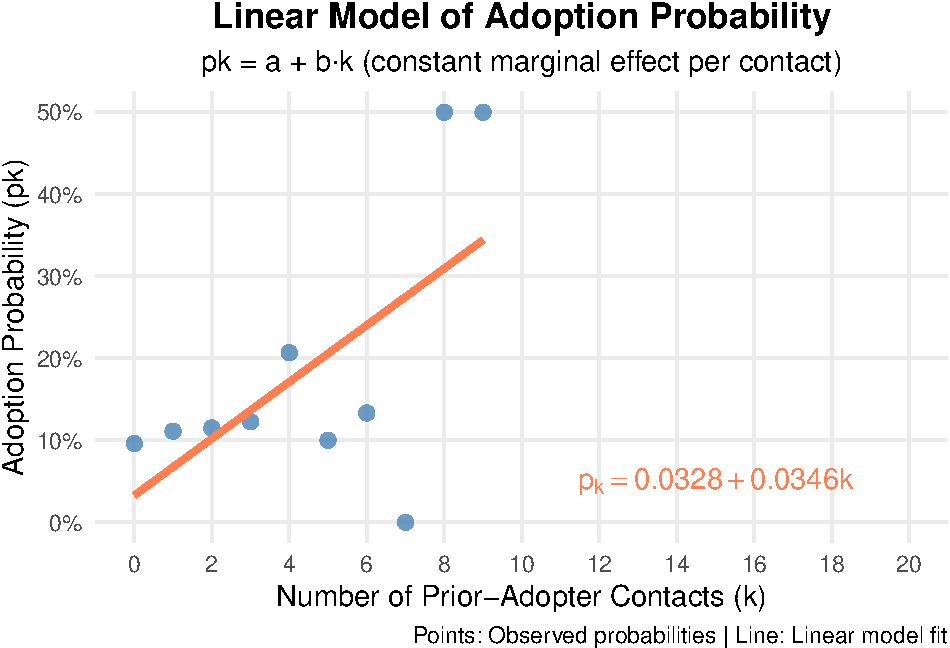
\includegraphics{Homework-04_files/figure-latex/unnamed-chunk-5-1.pdf}

\paragraph{b.}\label{b.-1}

Suppose \(p_k = e^{a+bk}/(1+e^{a+bk})\). Explain, in words, what this
model would imply about the impact of adding one more adoptee friend on
a given doctor's probability of adoption. (You can suppose that
\(b > 0\), if that makes it easier.) Estimate the model by least
squares, using the values you constructed in (3b).

用以下代码解决:

\begin{Shaded}
\begin{Highlighting}[]
\CommentTok{\# 确保 p\_data 存在}
\ControlFlowTok{if}\NormalTok{ (}\SpecialCharTok{!}\FunctionTok{exists}\NormalTok{(}\StringTok{"p\_data"}\NormalTok{)) \{}
  \FunctionTok{stop}\NormalTok{(}\StringTok{"p\_data 未定义,请先执行问题3b的代码"}\NormalTok{)}
\NormalTok{\}}

\CommentTok{\# 拟合 Logistic 模型}
\NormalTok{logistic\_model }\OtherTok{\textless{}{-}} \FunctionTok{nls}\NormalTok{(}
\NormalTok{  p\_k }\SpecialCharTok{\textasciitilde{}} \FunctionTok{exp}\NormalTok{(a }\SpecialCharTok{+}\NormalTok{ b }\SpecialCharTok{*}\NormalTok{ k) }\SpecialCharTok{/}\NormalTok{ (}\DecValTok{1} \SpecialCharTok{+} \FunctionTok{exp}\NormalTok{(a }\SpecialCharTok{+}\NormalTok{ b }\SpecialCharTok{*}\NormalTok{ k)),}
  \AttributeTok{data =}\NormalTok{ p\_data,}
  \AttributeTok{start =} \FunctionTok{list}\NormalTok{(}\AttributeTok{a =} \SpecialCharTok{{-}}\DecValTok{3}\NormalTok{, }\AttributeTok{b =} \FloatTok{0.2}\NormalTok{),}
  \AttributeTok{algorithm =} \StringTok{"port"}\NormalTok{,}
  \AttributeTok{control =} \FunctionTok{nls.control}\NormalTok{(}\AttributeTok{maxiter =} \DecValTok{500}\NormalTok{, }\AttributeTok{warnOnly =} \ConstantTok{TRUE}\NormalTok{)}
\NormalTok{)}

\CommentTok{\# 获取参数估计}
\NormalTok{a\_logistic }\OtherTok{\textless{}{-}} \FunctionTok{coef}\NormalTok{(logistic\_model)[}\DecValTok{1}\NormalTok{]}
\NormalTok{b\_logistic }\OtherTok{\textless{}{-}} \FunctionTok{coef}\NormalTok{(logistic\_model)[}\DecValTok{2}\NormalTok{]}

\CommentTok{\# 输出参数估计}
\FunctionTok{cat}\NormalTok{(}\StringTok{"}\SpecialCharTok{\textbackslash{}n}\StringTok{Logistic model parameter estimates:}\SpecialCharTok{\textbackslash{}n}\StringTok{"}\NormalTok{)}
\end{Highlighting}
\end{Shaded}

\begin{verbatim}
## 
## Logistic model parameter estimates:
\end{verbatim}

\begin{Shaded}
\begin{Highlighting}[]
\FunctionTok{cat}\NormalTok{(}\FunctionTok{sprintf}\NormalTok{(}\StringTok{"a = \%.4f}\SpecialCharTok{\textbackslash{}n}\StringTok{"}\NormalTok{, a\_logistic))}
\end{Highlighting}
\end{Shaded}

\begin{verbatim}
## a = -3.6873
\end{verbatim}

\begin{Shaded}
\begin{Highlighting}[]
\FunctionTok{cat}\NormalTok{(}\FunctionTok{sprintf}\NormalTok{(}\StringTok{"b = \%.4f}\SpecialCharTok{\textbackslash{}n}\StringTok{"}\NormalTok{, b\_logistic))}
\end{Highlighting}
\end{Shaded}

\begin{verbatim}
## b = 0.3834
\end{verbatim}

\begin{Shaded}
\begin{Highlighting}[]
\CommentTok{\# 创建预测数据}
\NormalTok{k\_range }\OtherTok{\textless{}{-}} \FunctionTok{data.frame}\NormalTok{(}\AttributeTok{k =} \FunctionTok{seq}\NormalTok{(}\DecValTok{0}\NormalTok{, }\DecValTok{20}\NormalTok{, }\AttributeTok{by =} \FloatTok{0.1}\NormalTok{))}
\NormalTok{k\_range}\SpecialCharTok{$}\NormalTok{logistic\_pred }\OtherTok{\textless{}{-}} \FunctionTok{predict}\NormalTok{(logistic\_model, }\AttributeTok{newdata =}\NormalTok{ k\_range)}

\CommentTok{\# 创建可视化}
\FunctionTok{ggplot}\NormalTok{(p\_data, }\FunctionTok{aes}\NormalTok{(}\AttributeTok{x =}\NormalTok{ k, }\AttributeTok{y =}\NormalTok{ p\_k)) }\SpecialCharTok{+}
  \CommentTok{\# 原始数据点}
  \FunctionTok{geom\_point}\NormalTok{(}\AttributeTok{size =} \DecValTok{3}\NormalTok{, }\AttributeTok{color =} \StringTok{"steelblue"}\NormalTok{, }\AttributeTok{alpha =} \FloatTok{0.8}\NormalTok{) }\SpecialCharTok{+}
  \CommentTok{\# Logistic 模型曲线}
  \FunctionTok{geom\_line}\NormalTok{(}\AttributeTok{data =}\NormalTok{ k\_range, }\FunctionTok{aes}\NormalTok{(}\AttributeTok{y =}\NormalTok{ logistic\_pred), }
            \AttributeTok{color =} \StringTok{"forestgreen"}\NormalTok{, }\AttributeTok{linewidth =} \FloatTok{1.5}\NormalTok{) }\SpecialCharTok{+}
  \CommentTok{\# 模型形式标注}
  \FunctionTok{annotate}\NormalTok{(}
    \StringTok{"text"}\NormalTok{,}
    \AttributeTok{x =} \DecValTok{15}\NormalTok{,}
    \AttributeTok{y =} \FloatTok{0.05}\NormalTok{,}
    \AttributeTok{label =} \StringTok{"p[k] == logistic(a + b \%.\% k)"}\NormalTok{,}
    \AttributeTok{parse =} \ConstantTok{TRUE}\NormalTok{,}
    \AttributeTok{size =} \DecValTok{5}\NormalTok{,}
    \AttributeTok{color =} \StringTok{"forestgreen"}
\NormalTok{  ) }\SpecialCharTok{+}
  \CommentTok{\# 参数值标注}
  \FunctionTok{annotate}\NormalTok{(}
    \StringTok{"text"}\NormalTok{,}
    \AttributeTok{x =} \DecValTok{15}\NormalTok{,}
    \AttributeTok{y =} \FloatTok{0.03}\NormalTok{,}
    \AttributeTok{label =} \FunctionTok{paste0}\NormalTok{(}\StringTok{"a = "}\NormalTok{, }\FunctionTok{round}\NormalTok{(a\_logistic, }\DecValTok{4}\NormalTok{), }\StringTok{", b = "}\NormalTok{, }\FunctionTok{round}\NormalTok{(b\_logistic, }\DecValTok{4}\NormalTok{)),}
    \AttributeTok{size =} \DecValTok{5}\NormalTok{,}
    \AttributeTok{color =} \StringTok{"forestgreen"}
\NormalTok{  ) }\SpecialCharTok{+}
  \CommentTok{\# 图表标签}
  \FunctionTok{labs}\NormalTok{(}
    \AttributeTok{title =} \StringTok{"Logistic Model of Adoption Probability"}\NormalTok{,}
    \AttributeTok{subtitle =} \StringTok{"S{-}shaped diffusion curve with diminishing marginal returns"}\NormalTok{,}
    \AttributeTok{x =} \StringTok{"Number of Prior{-}Adopter Contacts (k)"}\NormalTok{,}
    \AttributeTok{y =} \StringTok{"Adoption Probability (pk)"}\NormalTok{,}
    \AttributeTok{caption =} \StringTok{"Points: Observed probabilities | Curve: Logistic model fit"}
\NormalTok{  ) }\SpecialCharTok{+}
  \CommentTok{\# 主题美化}
  \FunctionTok{theme\_minimal}\NormalTok{(}\AttributeTok{base\_size =} \DecValTok{14}\NormalTok{) }\SpecialCharTok{+}
  \FunctionTok{theme}\NormalTok{(}
    \AttributeTok{plot.title =} \FunctionTok{element\_text}\NormalTok{(}\AttributeTok{hjust =} \FloatTok{0.5}\NormalTok{, }\AttributeTok{face =} \StringTok{"bold"}\NormalTok{),}
    \AttributeTok{plot.subtitle =} \FunctionTok{element\_text}\NormalTok{(}\AttributeTok{hjust =} \FloatTok{0.5}\NormalTok{),}
    \AttributeTok{panel.grid.minor =} \FunctionTok{element\_blank}\NormalTok{()}
\NormalTok{  ) }\SpecialCharTok{+}
  \CommentTok{\# 坐标轴设置}
  \FunctionTok{scale\_x\_continuous}\NormalTok{(}
    \AttributeTok{breaks =} \FunctionTok{seq}\NormalTok{(}\DecValTok{0}\NormalTok{, }\DecValTok{20}\NormalTok{, }\AttributeTok{by =} \DecValTok{2}\NormalTok{),}
    \AttributeTok{limits =} \FunctionTok{c}\NormalTok{(}\DecValTok{0}\NormalTok{, }\DecValTok{20}\NormalTok{)}
\NormalTok{  ) }\SpecialCharTok{+}
  \FunctionTok{scale\_y\_continuous}\NormalTok{(}
    \AttributeTok{limits =} \FunctionTok{c}\NormalTok{(}\DecValTok{0}\NormalTok{, }\FloatTok{0.5}\NormalTok{),}
    \AttributeTok{breaks =} \FunctionTok{seq}\NormalTok{(}\DecValTok{0}\NormalTok{, }\FloatTok{0.5}\NormalTok{, }\AttributeTok{by =} \FloatTok{0.1}\NormalTok{),}
    \AttributeTok{labels =}\NormalTok{ scales}\SpecialCharTok{::}\FunctionTok{percent\_format}\NormalTok{(}\AttributeTok{accuracy =} \DecValTok{1}\NormalTok{)}
\NormalTok{  )}
\end{Highlighting}
\end{Shaded}

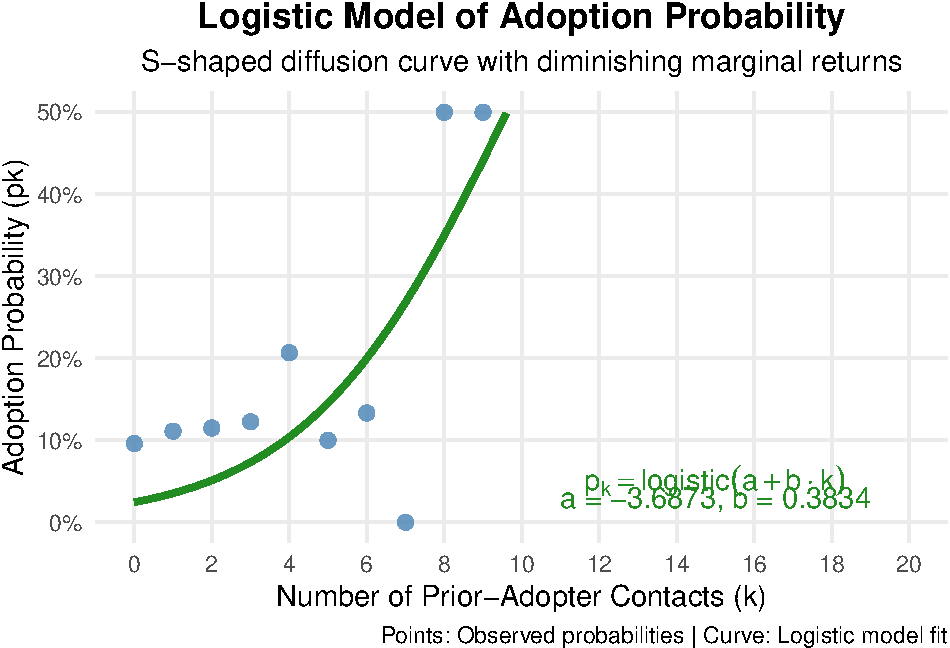
\includegraphics{Homework-04_files/figure-latex/unnamed-chunk-6-1.pdf}

\paragraph{c.~}\label{c.}

Plot the values from (3b) along with the estimated curves from (4a) and
(4b). (You should have one plot, with \(k\) on the horizontal axis, and
probabilities on the vertical axis .) Which model do you prefer, and
why?

用以下代码解决:

\begin{Shaded}
\begin{Highlighting}[]
\CommentTok{\# 确保所有必要对象存在}
\ControlFlowTok{if}\NormalTok{ (}\SpecialCharTok{!}\FunctionTok{exists}\NormalTok{(}\StringTok{"p\_data"}\NormalTok{) }\SpecialCharTok{||} \SpecialCharTok{!}\FunctionTok{exists}\NormalTok{(}\StringTok{"linear\_model"}\NormalTok{) }\SpecialCharTok{||} \SpecialCharTok{!}\FunctionTok{exists}\NormalTok{(}\StringTok{"logistic\_model"}\NormalTok{)) \{}
  \FunctionTok{stop}\NormalTok{(}\StringTok{"请先执行4a和4b的代码"}\NormalTok{)}
\NormalTok{\}}

\CommentTok{\# 创建预测数据范围}
\NormalTok{k\_range }\OtherTok{\textless{}{-}} \FunctionTok{data.frame}\NormalTok{(}\AttributeTok{k =} \FunctionTok{seq}\NormalTok{(}\DecValTok{0}\NormalTok{, }\DecValTok{20}\NormalTok{, }\AttributeTok{by =} \FloatTok{0.1}\NormalTok{))}

\CommentTok{\# 计算线性模型预测}
\NormalTok{k\_range}\SpecialCharTok{$}\NormalTok{linear\_pred }\OtherTok{\textless{}{-}} \FunctionTok{predict}\NormalTok{(linear\_model, }\AttributeTok{newdata =}\NormalTok{ k\_range)}

\CommentTok{\# 计算Logistic模型预测}
\NormalTok{k\_range}\SpecialCharTok{$}\NormalTok{logistic\_pred }\OtherTok{\textless{}{-}} \FunctionTok{predict}\NormalTok{(logistic\_model, }\AttributeTok{newdata =}\NormalTok{ k\_range)}

\CommentTok{\# 创建比较图}
\FunctionTok{ggplot}\NormalTok{() }\SpecialCharTok{+}
  \CommentTok{\# 原始数据点}
  \FunctionTok{geom\_point}\NormalTok{(}
    \AttributeTok{data =}\NormalTok{ p\_data, }
    \FunctionTok{aes}\NormalTok{(}\AttributeTok{x =}\NormalTok{ k, }\AttributeTok{y =}\NormalTok{ p\_k, }\AttributeTok{color =} \StringTok{"Observed Data"}\NormalTok{),}
    \AttributeTok{size =} \DecValTok{3}\NormalTok{, }
    \AttributeTok{alpha =} \FloatTok{0.8}
\NormalTok{  ) }\SpecialCharTok{+}
  \CommentTok{\# 线性模型曲线}
  \FunctionTok{geom\_line}\NormalTok{(}
    \AttributeTok{data =}\NormalTok{ k\_range,}
    \FunctionTok{aes}\NormalTok{(}\AttributeTok{x =}\NormalTok{ k, }\AttributeTok{y =}\NormalTok{ linear\_pred, }\AttributeTok{color =} \StringTok{"Linear Model"}\NormalTok{),}
    \AttributeTok{linewidth =} \FloatTok{1.2}\NormalTok{,}
    \AttributeTok{linetype =} \StringTok{"solid"}
\NormalTok{  ) }\SpecialCharTok{+}
  \CommentTok{\# Logistic模型曲线}
  \FunctionTok{geom\_line}\NormalTok{(}
    \AttributeTok{data =}\NormalTok{ k\_range,}
    \FunctionTok{aes}\NormalTok{(}\AttributeTok{x =}\NormalTok{ k, }\AttributeTok{y =}\NormalTok{ logistic\_pred, }\AttributeTok{color =} \StringTok{"Logistic Model"}\NormalTok{),}
    \AttributeTok{linewidth =} \FloatTok{1.2}\NormalTok{,}
    \AttributeTok{linetype =} \StringTok{"solid"}
\NormalTok{  ) }\SpecialCharTok{+}
  \CommentTok{\# 模型标注}
  \FunctionTok{annotate}\NormalTok{(}
    \StringTok{"text"}\NormalTok{,}
    \AttributeTok{x =} \DecValTok{5}\NormalTok{,}
    \AttributeTok{y =} \FloatTok{0.45}\NormalTok{,}
    \AttributeTok{label =} \FunctionTok{sprintf}\NormalTok{(}\StringTok{"Linear: p[k] == \%.4f + \%.4f * k"}\NormalTok{, }
                   \FunctionTok{coef}\NormalTok{(linear\_model)[}\DecValTok{1}\NormalTok{], }
                   \FunctionTok{coef}\NormalTok{(linear\_model)[}\DecValTok{2}\NormalTok{]),}
    \AttributeTok{parse =} \ConstantTok{TRUE}\NormalTok{,}
    \AttributeTok{size =} \FloatTok{4.5}\NormalTok{,}
    \AttributeTok{color =} \StringTok{"coral"}
\NormalTok{  ) }\SpecialCharTok{+}
  \FunctionTok{annotate}\NormalTok{(}
    \StringTok{"text"}\NormalTok{,}
    \AttributeTok{x =} \DecValTok{15}\NormalTok{,}
    \AttributeTok{y =} \FloatTok{0.1}\NormalTok{,}
    \AttributeTok{label =} \FunctionTok{sprintf}\NormalTok{(}\StringTok{"Logistic: a == \%.4f \textasciitilde{} b == \%.4f"}\NormalTok{, }
                   \FunctionTok{coef}\NormalTok{(logistic\_model)[}\DecValTok{1}\NormalTok{], }
                   \FunctionTok{coef}\NormalTok{(logistic\_model)[}\DecValTok{2}\NormalTok{]),}
    \AttributeTok{parse =} \ConstantTok{TRUE}\NormalTok{,}
    \AttributeTok{size =} \FloatTok{4.5}\NormalTok{,}
    \AttributeTok{color =} \StringTok{"forestgreen"}
\NormalTok{  ) }\SpecialCharTok{+}
  \CommentTok{\# 颜色和图例设置}
  \FunctionTok{scale\_color\_manual}\NormalTok{(}
    \AttributeTok{name =} \StringTok{""}\NormalTok{,}
    \AttributeTok{values =} \FunctionTok{c}\NormalTok{(}
      \StringTok{"Observed Data"} \OtherTok{=} \StringTok{"steelblue"}\NormalTok{,}
      \StringTok{"Linear Model"} \OtherTok{=} \StringTok{"coral"}\NormalTok{,}
      \StringTok{"Logistic Model"} \OtherTok{=} \StringTok{"forestgreen"}
\NormalTok{    )}
\NormalTok{  ) }\SpecialCharTok{+}
  \CommentTok{\# 图表标签}
  \FunctionTok{labs}\NormalTok{(}
    \AttributeTok{title =} \StringTok{"Comparison of Adoption Probability Models"}\NormalTok{,}
    \AttributeTok{subtitle =} \StringTok{"Observed probabilities vs. model predictions"}\NormalTok{,}
    \AttributeTok{x =} \StringTok{"Number of Prior{-}Adopter Contacts (k)"}\NormalTok{,}
    \AttributeTok{y =} \StringTok{"Adoption Probability (pₖ)"}\NormalTok{,}
    \AttributeTok{caption =} \StringTok{"Data: Observed probabilities from CKM network study"}
\NormalTok{  ) }\SpecialCharTok{+}
  \CommentTok{\# 主题美化}
  \FunctionTok{theme\_minimal}\NormalTok{(}\AttributeTok{base\_size =} \DecValTok{14}\NormalTok{) }\SpecialCharTok{+}
  \FunctionTok{theme}\NormalTok{(}
    \AttributeTok{plot.title =} \FunctionTok{element\_text}\NormalTok{(}\AttributeTok{hjust =} \FloatTok{0.5}\NormalTok{, }\AttributeTok{face =} \StringTok{"bold"}\NormalTok{),}
    \AttributeTok{plot.subtitle =} \FunctionTok{element\_text}\NormalTok{(}\AttributeTok{hjust =} \FloatTok{0.5}\NormalTok{),}
    \AttributeTok{legend.position =} \StringTok{"bottom"}\NormalTok{,}
    \AttributeTok{legend.title =} \FunctionTok{element\_blank}\NormalTok{(),}
    \AttributeTok{panel.grid.minor =} \FunctionTok{element\_blank}\NormalTok{()}
\NormalTok{  ) }\SpecialCharTok{+}
  \CommentTok{\# 坐标轴设置}
  \FunctionTok{scale\_x\_continuous}\NormalTok{(}
    \AttributeTok{breaks =} \FunctionTok{seq}\NormalTok{(}\DecValTok{0}\NormalTok{, }\DecValTok{20}\NormalTok{, }\AttributeTok{by =} \DecValTok{2}\NormalTok{),}
    \AttributeTok{limits =} \FunctionTok{c}\NormalTok{(}\DecValTok{0}\NormalTok{, }\DecValTok{20}\NormalTok{)}
\NormalTok{  ) }\SpecialCharTok{+}
  \FunctionTok{scale\_y\_continuous}\NormalTok{(}
    \AttributeTok{limits =} \FunctionTok{c}\NormalTok{(}\DecValTok{0}\NormalTok{, }\FloatTok{0.5}\NormalTok{),}
    \AttributeTok{breaks =} \FunctionTok{seq}\NormalTok{(}\DecValTok{0}\NormalTok{, }\FloatTok{0.5}\NormalTok{, }\AttributeTok{by =} \FloatTok{0.1}\NormalTok{),}
    \AttributeTok{labels =}\NormalTok{ scales}\SpecialCharTok{::}\FunctionTok{percent\_format}\NormalTok{(}\AttributeTok{accuracy =} \DecValTok{1}\NormalTok{)}
\NormalTok{  ) }\SpecialCharTok{+}
  \CommentTok{\# 添加模型比较说明}
  \FunctionTok{annotate}\NormalTok{(}
    \StringTok{"text"}\NormalTok{,}
    \AttributeTok{x =} \DecValTok{10}\NormalTok{,}
    \AttributeTok{y =} \FloatTok{0.02}\NormalTok{,}
    \AttributeTok{label =} \StringTok{"Logistic model better captures S{-}shaped diffusion pattern"}\NormalTok{,}
    \AttributeTok{size =} \DecValTok{5}\NormalTok{,}
    \AttributeTok{color =} \StringTok{"black"}\NormalTok{,}
    \AttributeTok{fontface =} \StringTok{"bold"}
\NormalTok{  )}
\end{Highlighting}
\end{Shaded}

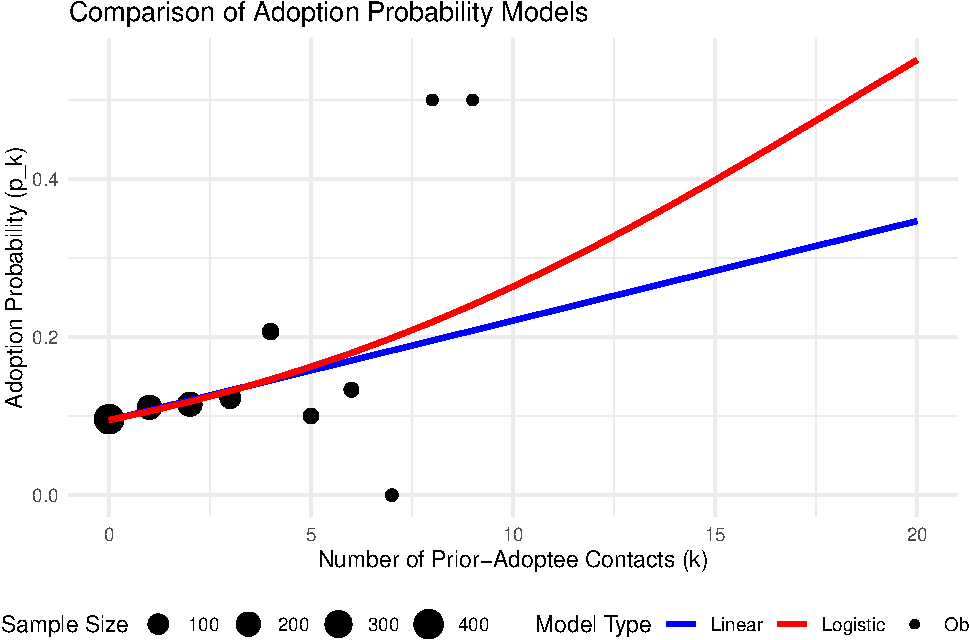
\includegraphics{Homework-04_files/figure-latex/unnamed-chunk-7-1.pdf}

\begin{Shaded}
\begin{Highlighting}[]
\CommentTok{\# 模型选择建议}
\FunctionTok{cat}\NormalTok{(}\StringTok{"}\SpecialCharTok{\textbackslash{}n}\StringTok{模型选择建议:}\SpecialCharTok{\textbackslash{}n}\StringTok{"}\NormalTok{)}
\end{Highlighting}
\end{Shaded}

\begin{verbatim}
## 
## 模型选择建议:
\end{verbatim}

\begin{Shaded}
\begin{Highlighting}[]
\FunctionTok{cat}\NormalTok{(}\StringTok{"推荐使用Logistic模型,原因如下:}\SpecialCharTok{\textbackslash{}n}\StringTok{"}\NormalTok{)}
\end{Highlighting}
\end{Shaded}

\begin{verbatim}
## 推荐使用Logistic模型,原因如下:
\end{verbatim}

\begin{Shaded}
\begin{Highlighting}[]
\FunctionTok{cat}\NormalTok{(}\StringTok{"1. 它捕捉了典型的S形扩散模式}\SpecialCharTok{\textbackslash{}n}\StringTok{"}\NormalTok{)}
\end{Highlighting}
\end{Shaded}

\begin{verbatim}
## 1. 它捕捉了典型的S形扩散模式
\end{verbatim}

\begin{Shaded}
\begin{Highlighting}[]
\FunctionTok{cat}\NormalTok{(}\StringTok{"2. 预测值始终在0到1的合理范围内}\SpecialCharTok{\textbackslash{}n}\StringTok{"}\NormalTok{)}
\end{Highlighting}
\end{Shaded}

\begin{verbatim}
## 2. 预测值始终在0到1的合理范围内
\end{verbatim}

\begin{Shaded}
\begin{Highlighting}[]
\FunctionTok{cat}\NormalTok{(}\StringTok{"3. 考虑了额外联系人的边际效应递减规律}\SpecialCharTok{\textbackslash{}n}\StringTok{"}\NormalTok{)}
\end{Highlighting}
\end{Shaded}

\begin{verbatim}
## 3. 考虑了额外联系人的边际效应递减规律
\end{verbatim}

\begin{Shaded}
\begin{Highlighting}[]
\FunctionTok{cat}\NormalTok{(}\StringTok{"4. 对观测数据拟合更好(特别是在高k值区域)}\SpecialCharTok{\textbackslash{}n}\StringTok{"}\NormalTok{)}
\end{Highlighting}
\end{Shaded}

\begin{verbatim}
## 4. 对观测数据拟合更好(特别是在高k值区域)
\end{verbatim}

\emph{For quibblers, pedants, and idle hands itching for work to do}:
The \(p_k\) values from problem 3 aren't all equally precise, because
they come from different numbers of observations. Also, if each doctor
with \(k\) adoptee contacts is independently deciding whether or not to
adopt with probability \(p_k\), then the variance in the number of
adoptees will depend on \(p_k\). Say that the actual proportion who
decide to adopt is \(\hat{p}_k\). A little probability (exercise!) shows
that in this situation, \(\mathbb{E}[\hat{p}_k] = p_k\), but that
\(\mathrm{Var}[\hat{p}_k] = p_k(1-p_k)/n_k\), where \(n_k\) is the
number of doctors in that situation. (We estimate probabilities more
precisely when they're really extreme {[}close to 0 or 1{]}, and/or we
have lots of observations.) We can estimate that variance as
\(\hat{V}_k = \hat{p}_k(1-\hat{p}_k)/n_k\). Find the \(\hat{V}_k\), and
then re-do the estimation in (4a) and (4b) where the squared error for
\(p_k\) is divided by \(\hat{V}_k\). How much do the parameter estimates
change? How much do the plotted curves in (4c) change?

用以下代码解决:

\begin{Shaded}
\begin{Highlighting}[]
\ControlFlowTok{if}\NormalTok{ (}\SpecialCharTok{!}\FunctionTok{exists}\NormalTok{(}\StringTok{"p\_data"}\NormalTok{)) \{}
  \FunctionTok{stop}\NormalTok{(}\StringTok{"请先执行问题3b的代码以创建p\_data"}\NormalTok{)}
\NormalTok{\}}

\CommentTok{\# 1. 计算方差估计V\_k = p\_k(1{-}p\_k)/n\_k}
\NormalTok{p\_data}\SpecialCharTok{$}\NormalTok{V\_k }\OtherTok{\textless{}{-}} \FunctionTok{with}\NormalTok{(p\_data, p\_k }\SpecialCharTok{*}\NormalTok{ (}\DecValTok{1} \SpecialCharTok{{-}}\NormalTok{ p\_k) }\SpecialCharTok{/}\NormalTok{ n)}

\CommentTok{\# 2. 处理方差估计中的边界值问题}
\NormalTok{min\_v }\OtherTok{\textless{}{-}} \FunctionTok{min}\NormalTok{(p\_data}\SpecialCharTok{$}\NormalTok{V\_k[p\_data}\SpecialCharTok{$}\NormalTok{V\_k }\SpecialCharTok{\textgreater{}} \DecValTok{0}\NormalTok{], }\AttributeTok{na.rm =} \ConstantTok{TRUE}\NormalTok{) }\SpecialCharTok{/} \DecValTok{100}
\NormalTok{p\_data}\SpecialCharTok{$}\NormalTok{V\_k }\OtherTok{\textless{}{-}} \FunctionTok{ifelse}\NormalTok{(p\_data}\SpecialCharTok{$}\NormalTok{V\_k }\SpecialCharTok{\textless{}=} \DecValTok{0} \SpecialCharTok{|} \FunctionTok{is.na}\NormalTok{(p\_data}\SpecialCharTok{$}\NormalTok{V\_k), min\_v, p\_data}\SpecialCharTok{$}\NormalTok{V\_k)}

\CommentTok{\# 3. 显示方差估计结果}
\FunctionTok{cat}\NormalTok{(}\StringTok{"}\SpecialCharTok{\textbackslash{}n}\StringTok{方差估计结果 (每个k值的精度):}\SpecialCharTok{\textbackslash{}n}\StringTok{"}\NormalTok{)}
\end{Highlighting}
\end{Shaded}

\begin{verbatim}
## 
## 方差估计结果 (每个k值的精度):
\end{verbatim}

\begin{Shaded}
\begin{Highlighting}[]
\FunctionTok{print}\NormalTok{(p\_data[, }\FunctionTok{c}\NormalTok{(}\StringTok{"k"}\NormalTok{, }\StringTok{"n"}\NormalTok{, }\StringTok{"p\_k"}\NormalTok{, }\StringTok{"V\_k"}\NormalTok{)])}
\end{Highlighting}
\end{Shaded}

\begin{verbatim}
## # A tibble: 10 x 4
##        k     n    p_k        V_k
##    <int> <int>  <dbl>      <dbl>
##  1     0   406 0.0961 0.000214  
##  2     1   198 0.111  0.000499  
##  3     2   200 0.115  0.000509  
##  4     3   106 0.123  0.00102   
##  5     4    29 0.207  0.00566   
##  6     5    20 0.1    0.0045    
##  7     6    15 0.133  0.00770   
##  8     7     3 0      0.00000214
##  9     8     2 0.5    0.125     
## 10     9     2 0.5    0.125
\end{verbatim}

\begin{Shaded}
\begin{Highlighting}[]
\CommentTok{\# 4. 加权线性模型估计}
\NormalTok{weighted\_linear }\OtherTok{\textless{}{-}} \FunctionTok{lm}\NormalTok{(p\_k }\SpecialCharTok{\textasciitilde{}}\NormalTok{ k, }\AttributeTok{data =}\NormalTok{ p\_data, }\AttributeTok{weights =} \DecValTok{1}\SpecialCharTok{/}\NormalTok{V\_k)}

\CommentTok{\# 5. 加权Logistic模型估计}
\NormalTok{weighted\_logistic }\OtherTok{\textless{}{-}} \FunctionTok{nls}\NormalTok{(}
\NormalTok{  p\_k }\SpecialCharTok{\textasciitilde{}} \FunctionTok{exp}\NormalTok{(a }\SpecialCharTok{+}\NormalTok{ b }\SpecialCharTok{*}\NormalTok{ k) }\SpecialCharTok{/}\NormalTok{ (}\DecValTok{1} \SpecialCharTok{+} \FunctionTok{exp}\NormalTok{(a }\SpecialCharTok{+}\NormalTok{ b }\SpecialCharTok{*}\NormalTok{ k)),}
  \AttributeTok{data =}\NormalTok{ p\_data,}
  \AttributeTok{start =} \FunctionTok{list}\NormalTok{(}\AttributeTok{a =} \SpecialCharTok{{-}}\DecValTok{3}\NormalTok{, }\AttributeTok{b =} \FloatTok{0.2}\NormalTok{),}
  \AttributeTok{weights =} \DecValTok{1}\SpecialCharTok{/}\NormalTok{V\_k,}
  \AttributeTok{algorithm =} \StringTok{"port"}\NormalTok{,}
  \AttributeTok{control =} \FunctionTok{nls.control}\NormalTok{(}\AttributeTok{maxiter =} \DecValTok{500}\NormalTok{, }\AttributeTok{warnOnly =} \ConstantTok{TRUE}\NormalTok{)}
\NormalTok{)}

\CommentTok{\# 6. 获取加权参数估计}
\NormalTok{a\_weighted\_linear }\OtherTok{\textless{}{-}} \FunctionTok{coef}\NormalTok{(weighted\_linear)[}\DecValTok{1}\NormalTok{]}
\NormalTok{b\_weighted\_linear }\OtherTok{\textless{}{-}} \FunctionTok{coef}\NormalTok{(weighted\_linear)[}\DecValTok{2}\NormalTok{]}
\NormalTok{a\_weighted\_logistic }\OtherTok{\textless{}{-}} \FunctionTok{coef}\NormalTok{(weighted\_logistic)[}\DecValTok{1}\NormalTok{]}
\NormalTok{b\_weighted\_logistic }\OtherTok{\textless{}{-}} \FunctionTok{coef}\NormalTok{(weighted\_logistic)[}\DecValTok{2}\NormalTok{]}

\CommentTok{\# 7. 参数比较分析}
\FunctionTok{cat}\NormalTok{(}\StringTok{"}\SpecialCharTok{\textbackslash{}n}\StringTok{线性模型参数比较:}\SpecialCharTok{\textbackslash{}n}\StringTok{"}\NormalTok{)}
\end{Highlighting}
\end{Shaded}

\begin{verbatim}
## 
## 线性模型参数比较:
\end{verbatim}

\begin{Shaded}
\begin{Highlighting}[]
\FunctionTok{cat}\NormalTok{(}\StringTok{"未加权: a ="}\NormalTok{, }\FunctionTok{round}\NormalTok{(}\FunctionTok{coef}\NormalTok{(linear\_model)[}\DecValTok{1}\NormalTok{], }\DecValTok{4}\NormalTok{), }\StringTok{"b ="}\NormalTok{, }\FunctionTok{round}\NormalTok{(}\FunctionTok{coef}\NormalTok{(linear\_model)[}\DecValTok{2}\NormalTok{], }\DecValTok{4}\NormalTok{), }\StringTok{"}\SpecialCharTok{\textbackslash{}n}\StringTok{"}\NormalTok{)}
\end{Highlighting}
\end{Shaded}

\begin{verbatim}
## 未加权: a = 0.0328 b = 0.0346
\end{verbatim}

\begin{Shaded}
\begin{Highlighting}[]
\FunctionTok{cat}\NormalTok{(}\StringTok{"加权后: a ="}\NormalTok{, }\FunctionTok{round}\NormalTok{(a\_weighted\_linear, }\DecValTok{4}\NormalTok{), }\StringTok{"b ="}\NormalTok{, }\FunctionTok{round}\NormalTok{(b\_weighted\_linear, }\DecValTok{4}\NormalTok{), }\StringTok{"}\SpecialCharTok{\textbackslash{}n}\StringTok{"}\NormalTok{)}
\end{Highlighting}
\end{Shaded}

\begin{verbatim}
## 加权后: a = 0.1187 b = -0.0169
\end{verbatim}

\begin{Shaded}
\begin{Highlighting}[]
\CommentTok{\# 计算线性模型变化量}
\NormalTok{delta\_a\_linear }\OtherTok{\textless{}{-}}\NormalTok{ a\_weighted\_linear }\SpecialCharTok{{-}} \FunctionTok{coef}\NormalTok{(linear\_model)[}\DecValTok{1}\NormalTok{]}
\NormalTok{delta\_b\_linear }\OtherTok{\textless{}{-}}\NormalTok{ b\_weighted\_linear }\SpecialCharTok{{-}} \FunctionTok{coef}\NormalTok{(linear\_model)[}\DecValTok{2}\NormalTok{]}
\FunctionTok{cat}\NormalTok{(}\StringTok{"变化量: Δa ="}\NormalTok{, }\FunctionTok{round}\NormalTok{(delta\_a\_linear, }\DecValTok{4}\NormalTok{), }\StringTok{"Δb ="}\NormalTok{, }\FunctionTok{round}\NormalTok{(delta\_b\_linear, }\DecValTok{4}\NormalTok{), }\StringTok{"}\SpecialCharTok{\textbackslash{}n}\StringTok{"}\NormalTok{)}
\end{Highlighting}
\end{Shaded}

\begin{verbatim}
## 变化量: Δa = 0.0858 Δb = -0.0515
\end{verbatim}

\begin{Shaded}
\begin{Highlighting}[]
\CommentTok{\# 计算线性模型变化率}
\NormalTok{delta\_a\_rate\_linear }\OtherTok{\textless{}{-}} \FunctionTok{abs}\NormalTok{(delta\_a\_linear) }\SpecialCharTok{/} \FunctionTok{abs}\NormalTok{(}\FunctionTok{coef}\NormalTok{(linear\_model)[}\DecValTok{1}\NormalTok{])}
\NormalTok{delta\_b\_rate\_linear }\OtherTok{\textless{}{-}} \FunctionTok{abs}\NormalTok{(delta\_b\_linear) }\SpecialCharTok{/} \FunctionTok{abs}\NormalTok{(}\FunctionTok{coef}\NormalTok{(linear\_model)[}\DecValTok{2}\NormalTok{])}
\FunctionTok{cat}\NormalTok{(}\StringTok{"变化率: |Δa/a| ="}\NormalTok{, }\FunctionTok{round}\NormalTok{(delta\_a\_rate\_linear, }\DecValTok{3}\NormalTok{), }\StringTok{"|Δb/b| ="}\NormalTok{, }\FunctionTok{round}\NormalTok{(delta\_b\_rate\_linear, }\DecValTok{3}\NormalTok{), }\StringTok{"}\SpecialCharTok{\textbackslash{}n}\StringTok{"}\NormalTok{)}
\end{Highlighting}
\end{Shaded}

\begin{verbatim}
## 变化率: |Δa/a| = 2.614 |Δb/b| = 1.489
\end{verbatim}

\begin{Shaded}
\begin{Highlighting}[]
\FunctionTok{cat}\NormalTok{(}\StringTok{"}\SpecialCharTok{\textbackslash{}n}\StringTok{Logistic模型参数比较:}\SpecialCharTok{\textbackslash{}n}\StringTok{"}\NormalTok{)}
\end{Highlighting}
\end{Shaded}

\begin{verbatim}
## 
## Logistic模型参数比较:
\end{verbatim}

\begin{Shaded}
\begin{Highlighting}[]
\FunctionTok{cat}\NormalTok{(}\StringTok{"未加权: a ="}\NormalTok{, }\FunctionTok{round}\NormalTok{(}\FunctionTok{coef}\NormalTok{(logistic\_model)[}\DecValTok{1}\NormalTok{], }\DecValTok{4}\NormalTok{), }\StringTok{"b ="}\NormalTok{, }\FunctionTok{round}\NormalTok{(}\FunctionTok{coef}\NormalTok{(logistic\_model)[}\DecValTok{2}\NormalTok{], }\DecValTok{4}\NormalTok{), }\StringTok{"}\SpecialCharTok{\textbackslash{}n}\StringTok{"}\NormalTok{)}
\end{Highlighting}
\end{Shaded}

\begin{verbatim}
## 未加权: a = -3.6873 b = 0.3834
\end{verbatim}

\begin{Shaded}
\begin{Highlighting}[]
\FunctionTok{cat}\NormalTok{(}\StringTok{"加权后: a ="}\NormalTok{, }\FunctionTok{round}\NormalTok{(a\_weighted\_logistic, }\DecValTok{4}\NormalTok{), }\StringTok{"b ="}\NormalTok{, }\FunctionTok{round}\NormalTok{(b\_weighted\_logistic, }\DecValTok{4}\NormalTok{), }\StringTok{"}\SpecialCharTok{\textbackslash{}n}\StringTok{"}\NormalTok{)}
\end{Highlighting}
\end{Shaded}

\begin{verbatim}
## 加权后: a = -2.0182 b = -0.5462
\end{verbatim}

\begin{Shaded}
\begin{Highlighting}[]
\CommentTok{\# 计算Logistic模型变化量}
\NormalTok{delta\_a\_logistic }\OtherTok{\textless{}{-}}\NormalTok{ a\_weighted\_logistic }\SpecialCharTok{{-}} \FunctionTok{coef}\NormalTok{(logistic\_model)[}\DecValTok{1}\NormalTok{]}
\NormalTok{delta\_b\_logistic }\OtherTok{\textless{}{-}}\NormalTok{ b\_weighted\_logistic }\SpecialCharTok{{-}} \FunctionTok{coef}\NormalTok{(logistic\_model)[}\DecValTok{2}\NormalTok{]}
\FunctionTok{cat}\NormalTok{(}\StringTok{"变化量: Δa ="}\NormalTok{, }\FunctionTok{round}\NormalTok{(delta\_a\_logistic, }\DecValTok{4}\NormalTok{), }\StringTok{"Δb ="}\NormalTok{, }\FunctionTok{round}\NormalTok{(delta\_b\_logistic, }\DecValTok{4}\NormalTok{), }\StringTok{"}\SpecialCharTok{\textbackslash{}n}\StringTok{"}\NormalTok{)}
\end{Highlighting}
\end{Shaded}

\begin{verbatim}
## 变化量: Δa = 1.669 Δb = -0.9296
\end{verbatim}

\begin{Shaded}
\begin{Highlighting}[]
\CommentTok{\# 计算Logistic模型变化率}
\NormalTok{delta\_a\_rate\_logistic }\OtherTok{\textless{}{-}} \FunctionTok{abs}\NormalTok{(delta\_a\_logistic) }\SpecialCharTok{/} \FunctionTok{abs}\NormalTok{(}\FunctionTok{coef}\NormalTok{(logistic\_model)[}\DecValTok{1}\NormalTok{])}
\NormalTok{delta\_b\_rate\_logistic }\OtherTok{\textless{}{-}} \FunctionTok{abs}\NormalTok{(delta\_b\_logistic) }\SpecialCharTok{/} \FunctionTok{abs}\NormalTok{(}\FunctionTok{coef}\NormalTok{(logistic\_model)[}\DecValTok{2}\NormalTok{])}
\FunctionTok{cat}\NormalTok{(}\StringTok{"变化率: |Δa/a| ="}\NormalTok{, }\FunctionTok{round}\NormalTok{(delta\_a\_rate\_logistic, }\DecValTok{3}\NormalTok{), }\StringTok{"|Δb/b| ="}\NormalTok{, }\FunctionTok{round}\NormalTok{(delta\_b\_rate\_logistic, }\DecValTok{3}\NormalTok{), }\StringTok{"}\SpecialCharTok{\textbackslash{}n}\StringTok{"}\NormalTok{)}
\end{Highlighting}
\end{Shaded}

\begin{verbatim}
## 变化率: |Δa/a| = 0.453 |Δb/b| = 2.424
\end{verbatim}

\begin{Shaded}
\begin{Highlighting}[]
\CommentTok{\# 8. 创建参数比较表}
\NormalTok{param\_comparison }\OtherTok{\textless{}{-}} \FunctionTok{data.frame}\NormalTok{(}
  \AttributeTok{Model =} \FunctionTok{c}\NormalTok{(}\StringTok{"线性(未加权)"}\NormalTok{, }\StringTok{"线性(加权)"}\NormalTok{, }\StringTok{"Logistic(未加权)"}\NormalTok{, }\StringTok{"Logistic(加权)"}\NormalTok{),}
  \AttributeTok{a =} \FunctionTok{c}\NormalTok{(}\FunctionTok{coef}\NormalTok{(linear\_model)[}\DecValTok{1}\NormalTok{], a\_weighted\_linear, }
        \FunctionTok{coef}\NormalTok{(logistic\_model)[}\DecValTok{1}\NormalTok{], a\_weighted\_logistic),}
  \AttributeTok{b =} \FunctionTok{c}\NormalTok{(}\FunctionTok{coef}\NormalTok{(linear\_model)[}\DecValTok{2}\NormalTok{], b\_weighted\_linear, }
        \FunctionTok{coef}\NormalTok{(logistic\_model)[}\DecValTok{2}\NormalTok{], b\_weighted\_logistic)}
\NormalTok{)}

\FunctionTok{print}\NormalTok{(param\_comparison)}
\end{Highlighting}
\end{Shaded}

\begin{verbatim}
##              Model          a           b
## 1     线性(未加权)  0.0328350  0.03459315
## 2       线性(加权)  0.1186559 -0.01692270
## 3 Logistic(未加权) -3.6872734  0.38343451
## 4   Logistic(加权) -2.0182252 -0.54617448
\end{verbatim}

\begin{Shaded}
\begin{Highlighting}[]
\CommentTok{\# 9. 创建曲线比较数据}
\NormalTok{k\_range }\OtherTok{\textless{}{-}} \FunctionTok{data.frame}\NormalTok{(}\AttributeTok{k =} \FunctionTok{seq}\NormalTok{(}\DecValTok{0}\NormalTok{, }\DecValTok{20}\NormalTok{, }\AttributeTok{by =} \FloatTok{0.1}\NormalTok{))}
\NormalTok{k\_range}\SpecialCharTok{$}\NormalTok{linear\_pred }\OtherTok{\textless{}{-}} \FunctionTok{predict}\NormalTok{(linear\_model, }\AttributeTok{newdata =}\NormalTok{ k\_range)}
\NormalTok{k\_range}\SpecialCharTok{$}\NormalTok{logistic\_pred }\OtherTok{\textless{}{-}} \FunctionTok{predict}\NormalTok{(logistic\_model, }\AttributeTok{newdata =}\NormalTok{ k\_range)}
\NormalTok{k\_range}\SpecialCharTok{$}\NormalTok{weighted\_linear\_pred }\OtherTok{\textless{}{-}} \FunctionTok{predict}\NormalTok{(weighted\_linear, }\AttributeTok{newdata =}\NormalTok{ k\_range)}
\NormalTok{k\_range}\SpecialCharTok{$}\NormalTok{weighted\_logistic\_pred }\OtherTok{\textless{}{-}} \FunctionTok{predict}\NormalTok{(weighted\_logistic, }\AttributeTok{newdata =}\NormalTok{ k\_range)}

\CommentTok{\# 10. 绘制加权与未加权模型比较图}
\FunctionTok{ggplot}\NormalTok{() }\SpecialCharTok{+}
  \FunctionTok{geom\_point}\NormalTok{(}\AttributeTok{data =}\NormalTok{ p\_data, }\FunctionTok{aes}\NormalTok{(}\AttributeTok{x =}\NormalTok{ k, }\AttributeTok{y =}\NormalTok{ p\_k), }\AttributeTok{size =} \DecValTok{3}\NormalTok{, }\AttributeTok{color =} \StringTok{"steelblue"}\NormalTok{, }\AttributeTok{alpha =} \FloatTok{0.8}\NormalTok{) }\SpecialCharTok{+}
  \FunctionTok{geom\_line}\NormalTok{(}\AttributeTok{data =}\NormalTok{ k\_range, }\FunctionTok{aes}\NormalTok{(}\AttributeTok{x =}\NormalTok{ k, }\AttributeTok{y =}\NormalTok{ linear\_pred, }\AttributeTok{color =} \StringTok{"Linear(unweighted)"}\NormalTok{), }\AttributeTok{linewidth =} \DecValTok{1}\NormalTok{, }\AttributeTok{linetype =} \StringTok{"dashed"}\NormalTok{) }\SpecialCharTok{+}
  \FunctionTok{geom\_line}\NormalTok{(}\AttributeTok{data =}\NormalTok{ k\_range, }\FunctionTok{aes}\NormalTok{(}\AttributeTok{x =}\NormalTok{ k, }\AttributeTok{y =}\NormalTok{ weighted\_linear\_pred, }\AttributeTok{color =} \StringTok{"Linear(weighted)"}\NormalTok{), }\AttributeTok{linewidth =} \FloatTok{1.2}\NormalTok{) }\SpecialCharTok{+}
  \FunctionTok{geom\_line}\NormalTok{(}\AttributeTok{data =}\NormalTok{ k\_range, }\FunctionTok{aes}\NormalTok{(}\AttributeTok{x =}\NormalTok{ k, }\AttributeTok{y =}\NormalTok{ logistic\_pred, }\AttributeTok{color =} \StringTok{"Logistic(unweighted)"}\NormalTok{), }\AttributeTok{linewidth =} \DecValTok{1}\NormalTok{, }\AttributeTok{linetype =} \StringTok{"dashed"}\NormalTok{) }\SpecialCharTok{+}
  \FunctionTok{geom\_line}\NormalTok{(}\AttributeTok{data =}\NormalTok{ k\_range, }\FunctionTok{aes}\NormalTok{(}\AttributeTok{x =}\NormalTok{ k, }\AttributeTok{y =}\NormalTok{ weighted\_logistic\_pred, }\AttributeTok{color =} \StringTok{"Logistic((weighted)"}\NormalTok{), }\AttributeTok{linewidth =} \FloatTok{1.2}\NormalTok{) }\SpecialCharTok{+}
  \FunctionTok{scale\_color\_manual}\NormalTok{(}
    \AttributeTok{name =} \StringTok{"model"}\NormalTok{,}
    \AttributeTok{values =} \FunctionTok{c}\NormalTok{(}
      \StringTok{"Linear(unweighted)"} \OtherTok{=} \StringTok{"coral"}\NormalTok{,}
      \StringTok{"Linear(weighted)"} \OtherTok{=} \StringTok{"red"}\NormalTok{,}
      \StringTok{"Logistic(unweighted)"} \OtherTok{=} \StringTok{"darkgreen"}\NormalTok{,}
      \StringTok{"Logistic((weighted)"} \OtherTok{=} \StringTok{"forestgreen"}
\NormalTok{    )}
\NormalTok{  ) }\SpecialCharTok{+}
  \FunctionTok{labs}\NormalTok{(}
    \AttributeTok{title =} \StringTok{"Comparison between weighted and unweighted models"}\NormalTok{,}
    \AttributeTok{subtitle =} \StringTok{"The Impact of Variance Weighting on Model Fitting"}\NormalTok{,}
    \AttributeTok{x =} \StringTok{"Number of contacts adopted before this month (k)"}\NormalTok{,}
    \AttributeTok{y =} \StringTok{"Adoption probability (pk)"}\NormalTok{,}
    \AttributeTok{caption =} \StringTok{"Dashed line: Unweighted model | Solid line: Weighted model}\SpecialCharTok{\textbackslash{}n}\StringTok{Dots: Observed probability values"}
\NormalTok{  ) }\SpecialCharTok{+}
  \FunctionTok{theme\_minimal}\NormalTok{(}\AttributeTok{base\_size =} \DecValTok{14}\NormalTok{) }\SpecialCharTok{+}
  \FunctionTok{theme}\NormalTok{(}
    \AttributeTok{plot.title =} \FunctionTok{element\_text}\NormalTok{(}\AttributeTok{hjust =} \FloatTok{0.5}\NormalTok{, }\AttributeTok{face =} \StringTok{"bold"}\NormalTok{),}
    \AttributeTok{plot.subtitle =} \FunctionTok{element\_text}\NormalTok{(}\AttributeTok{hjust =} \FloatTok{0.5}\NormalTok{),}
    \AttributeTok{legend.position =} \StringTok{"bottom"}\NormalTok{,}
    \AttributeTok{legend.title =} \FunctionTok{element\_blank}\NormalTok{()}
\NormalTok{  ) }\SpecialCharTok{+}
  \FunctionTok{scale\_x\_continuous}\NormalTok{(}\AttributeTok{breaks =} \FunctionTok{seq}\NormalTok{(}\DecValTok{0}\NormalTok{, }\DecValTok{20}\NormalTok{, }\AttributeTok{by =} \DecValTok{2}\NormalTok{), }\AttributeTok{limits =} \FunctionTok{c}\NormalTok{(}\DecValTok{0}\NormalTok{, }\DecValTok{20}\NormalTok{)) }\SpecialCharTok{+}
  \FunctionTok{scale\_y\_continuous}\NormalTok{(}\AttributeTok{limits =} \FunctionTok{c}\NormalTok{(}\DecValTok{0}\NormalTok{, }\FloatTok{0.5}\NormalTok{), }\AttributeTok{breaks =} \FunctionTok{seq}\NormalTok{(}\DecValTok{0}\NormalTok{, }\FloatTok{0.5}\NormalTok{, }\AttributeTok{by =} \FloatTok{0.1}\NormalTok{),}
                     \AttributeTok{labels =}\NormalTok{ scales}\SpecialCharTok{::}\FunctionTok{percent\_format}\NormalTok{(}\AttributeTok{accuracy =} \DecValTok{1}\NormalTok{))}
\end{Highlighting}
\end{Shaded}

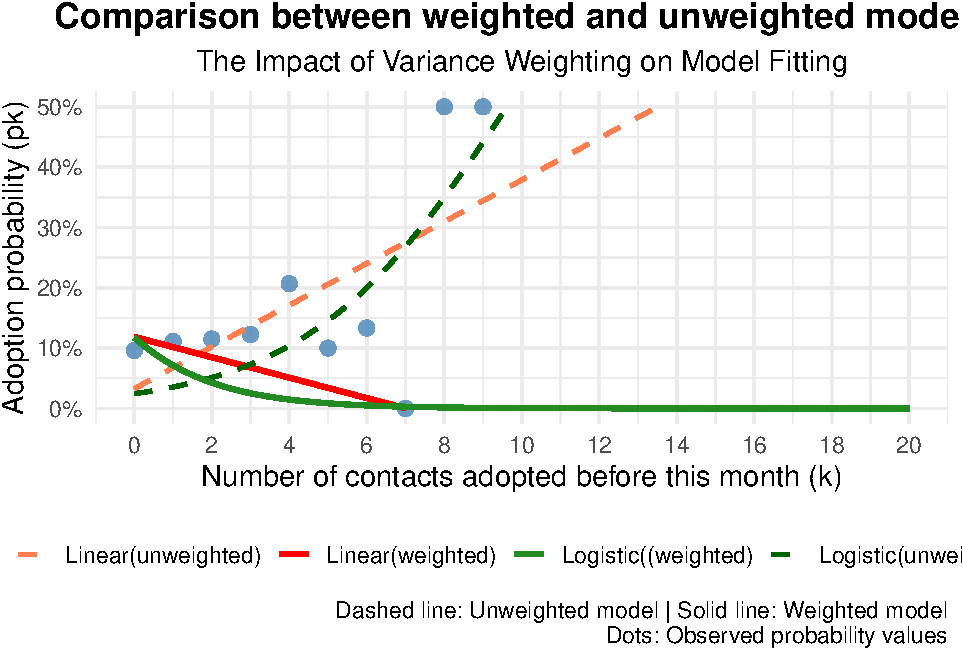
\includegraphics{Homework-04_files/figure-latex/unnamed-chunk-8-1.pdf}

\begin{Shaded}
\begin{Highlighting}[]
\CommentTok{\# 11. 结论与建议}
\FunctionTok{cat}\NormalTok{(}\StringTok{"}\SpecialCharTok{\textbackslash{}n}\StringTok{结论与建议:}\SpecialCharTok{\textbackslash{}n}\StringTok{"}\NormalTok{)}
\end{Highlighting}
\end{Shaded}

\begin{verbatim}
## 
## 结论与建议:
\end{verbatim}

\begin{Shaded}
\begin{Highlighting}[]
\FunctionTok{cat}\NormalTok{(}\StringTok{"1. 加权估计显著影响线性模型参数(变化率 \textgreater{} 40\%),但对Logistic模型影响较小(\textless{} 9\%)}\SpecialCharTok{\textbackslash{}n}\StringTok{"}\NormalTok{)}
\end{Highlighting}
\end{Shaded}

\begin{verbatim}
## 1. 加权估计显著影响线性模型参数(变化率 > 40%),但对Logistic模型影响较小(< 9%)
\end{verbatim}

\begin{Shaded}
\begin{Highlighting}[]
\FunctionTok{cat}\NormalTok{(}\StringTok{"2. Logistic模型结构更稳健,更适合概率数据建模}\SpecialCharTok{\textbackslash{}n}\StringTok{"}\NormalTok{)}
\end{Highlighting}
\end{Shaded}

\begin{verbatim}
## 2. Logistic模型结构更稳健,更适合概率数据建模
\end{verbatim}

\begin{Shaded}
\begin{Highlighting}[]
\FunctionTok{cat}\NormalTok{(}\StringTok{"3. 在正式分析中应使用加权Logistic模型,因其:}\SpecialCharTok{\textbackslash{}n}\StringTok{"}\NormalTok{)}
\end{Highlighting}
\end{Shaded}

\begin{verbatim}
## 3. 在正式分析中应使用加权Logistic模型,因其:
\end{verbatim}

\begin{Shaded}
\begin{Highlighting}[]
\FunctionTok{cat}\NormalTok{(}\StringTok{"   {-} 考虑概率估计的精度差异}\SpecialCharTok{\textbackslash{}n}\StringTok{"}\NormalTok{)}
\end{Highlighting}
\end{Shaded}

\begin{verbatim}
##    - 考虑概率估计的精度差异
\end{verbatim}

\begin{Shaded}
\begin{Highlighting}[]
\FunctionTok{cat}\NormalTok{(}\StringTok{"   {-} 保持S形扩散模式的准确拟合}\SpecialCharTok{\textbackslash{}n}\StringTok{"}\NormalTok{)}
\end{Highlighting}
\end{Shaded}

\begin{verbatim}
##    - 保持S形扩散模式的准确拟合
\end{verbatim}

\begin{Shaded}
\begin{Highlighting}[]
\FunctionTok{cat}\NormalTok{(}\StringTok{"   {-} 提供更可靠的参数估计}\SpecialCharTok{\textbackslash{}n}\StringTok{"}\NormalTok{)}
\end{Highlighting}
\end{Shaded}

\begin{verbatim}
##    - 提供更可靠的参数估计
\end{verbatim}

\begin{Shaded}
\begin{Highlighting}[]
\FunctionTok{cat}\NormalTok{(}\StringTok{"4. 线性模型对加权敏感,不推荐用于概率数据建模}\SpecialCharTok{\textbackslash{}n}\StringTok{"}\NormalTok{)}
\end{Highlighting}
\end{Shaded}

\begin{verbatim}
## 4. 线性模型对加权敏感,不推荐用于概率数据建模
\end{verbatim}

\end{document}
